\newcommand{\hsbind}{\mathbin{\gg\!=}}
\newcommand{\kleisli}{\mathbin{>\!=\!\!>}}
\newcommand{\comp}{\mathbin{\circ}}

\newcommand{\opl}[1]{\mathbin{\ll\!\!#1}}
\newcommand{\opll}[1]{\mathbin{\lll\!\!#1}}
\newcommand{\opr}[1]{\mathbin{#1\!\!\gg}}
\newcommand{\oplr}[1]{\mathbin{\ll\!\!#1\!\!\gg}}

\newcommand{\apl}{\opl{\cdot}}
\newcommand{\apll}{\opll{\cdot}}
\newcommand{\apr}{\opr{\cdot}}
\newcommand{\aplr}{\oplr{\cdot}}
\newcommand{\eql}{\opl{=}}
\newcommand{\eqr}{\opr{=}}
\newcommand{\eqlr}{\oplr{=}}
\newcommand{\andl}{\opl{\land}}
\newcommand{\andr}{\opr{\land}}
\newcommand{\andlr}{\oplr{\land}}
\newcommand{\impl}{\opl{\to}}
\newcommand{\impr}{\opr{\to}}
\newcommand{\implr}{\oplr{\to}}
\newcommand{\orl}{\opl{\lor}}
\newcommand{\orr}{\opr{\lor}}
\newcommand{\orlr}{\oplr{\lor}}
\newcommand{\notr}{\opr{\lnot}}
\newcommand{\somelr}{\oplr{\_}}

\newcommand{\cons}{\mathbin{::}}
\newcommand{\cat}{\mathbin{+\mkern-10mu+}}
\newcommand{\nil}{\mathrm{nil}}


\newcommand{\abs}[1]{\textsc{#1}}
\newcommand{\obj}[1]{\textbf{#1}}
\newcommand{\sem}[1]{\llbracket #1 \rrbracket}
\newcommand{\lex}[2]{\sem{\abs{#1}} &= #2}

\newcommand{\dand}{\mathbin{\overline{\land}}}
\newcommand{\dnot}{\mathop{\overline{\lnot}}}
\newcommand{\dor}{\mathop{\overline{\lor}}}
\newcommand{\dimp}{\mathbin{\overline{\to}}}
\newcommand{\dexists}{\mathop{\overline{\exists}}}
\newcommand{\existsr}{\mathop{\exists_\gg}}
\newcommand{\dforall}{\mathop{\overline{\forall}}}

\newcommand{\limp}{\mathbin{{-}\mkern-3.5mu{\circ}}}

\newcommand{\llbparenthesis}{\vcenter{\hbox{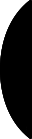
\includegraphics{symbols/llbparenthesis.png}}}}
\robustify{\llbparenthesis}
\newcommand{\rrbparenthesis}{\vcenter{\hbox{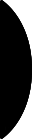
\includegraphics{symbols/rrbparenthesis.png}}}}
\robustify{\rrbparenthesis}
\newcommand{\lban}{\llparenthesis \,}
\newcommand{\rban}{\, \rrparenthesis}
\newcommand{\lbban}{\llbparenthesis \,}
\newcommand{\rbban}{\, \rrbparenthesis}
\newcommand{\banana}[1]{\lban #1 \rban}
\newcommand{\bbanana}[1]{\lbban #1 \rbban}
\newcommand{\cherry}{\text{\rotatebox[origin=c]{270}{$\limp$}}}

\newcommand{\lam}[2]{\lambda #1.\, #2}
\newcommand{\ap}[2]{#1\,#2}
\newcommand{\app}[3]{\ap{\ap{#1}{#2}}{#3}}
\newcommand{\appp}[4]{\ap{\ap{\ap{#1}{#2}}{#3}}{#4}}
\newcommand{\op}[1]{\mathtt{#1}}
\newcommand{\onto}[1]{#1 \mathalpha{:\,}}
\newcommand{\typedop}[3]{\op{#1} : #2 \rightarrowtail #3}
\newcommand{\typedopg}[3]{#1 : #2 \rightarrowtail #3}
\newcommand{\row}[2]{\{ #1 \mathrel{|} #2 \}}

\newcommand{\CC}{\mathcal{C}}
\newcommand{\BB}{\mathcal{B}}
\newcommand{\FF}{\mathcal{F}}
\newcommand{\XX}{\mathcal{X}}
\newcommand{\EE}{\mathcal{E}}
\newcommand{\TT}{\mathcal{T}}
\newcommand{\PP}{\mathcal{P}}
\newcommand{\ZZ}{\mathcal{Z}}
\newcommand{\II}{\mathcal{I}}
\newcommand{\AAA}{\mathcal{A}}
\newcommand{\RR}{\mathcal{R}}
\newcommand{\DD}{\mathcal{D}}

\newcommand{\FV}{\operatorname{FV}}

\newcommand{\subst}[3]{#1[#2 \coloneqq #3]}
\newcommand{\substt}[5]{#1[#2 \coloneqq #3, #4 \coloneqq #5]}

\newcommand{\syntclos}[1]{\mathbin{[#1]}}

\newtheorem{theorem}{Theorem}
\newtheorem{property}[theorem]{Property}
\newtheorem{observation}[theorem]{Observation}
\newtheorem{corollary}[theorem]{Corollary}
\newtheorem{lemma}[theorem]{Lemma}
\newtheorem{proposition}[theorem]{Proposition}
\newtheorem{law}[theorem]{Law}
\newtheorem{definition}[theorem]{Definition}
\newtheorem{notation}[theorem]{Notation}
\numberwithin{theorem}{section}

\newcommand{\cibanana}{\banana{(\onto{\op{op}_i} M_i)_{i \in I},\ \onto{\eta} M_\eta}}
\newcommand{\cdbanana}{\banana{\onto{\op{op}_1} M_1,\ \dots,\ \onto{\op{op}_n} M_n,\ \onto{\eta} M_\eta}}

\newcommand{\cibbanana}{\bbanana{(\onto{\op{op}_i} M_i)_{i \in I},\ \onto{\eta} M_\eta}}

\newcommand{\TODO}[1]{\textcolor{red}{\textbf{TODO}: #1}}

\newcommand{\relR}{\mathbin{R}}

\newcommand{\swap}{\mathbin{\textbf{swap}}}

\newcommand{\tto}{\twoheadrightarrow}

\mathchardef\mhyphen="2D

\newcommand{\pair}[2]{\left<#1, #2\right>}
\newcommand{\inl}{\operatorname{inl}}
\newcommand{\inr}{\operatorname{inr}}
\newcommand{\case}[5]{\text{\textbf{case} $#1$ \textbf{of} $\{ \ap{\inl}{#2} \to #3;\ \ap{\inr}{#4} \to #5 \}$}}
\newcommand{\casenl}[5]{\text{\textbf{case} $#1$ \textbf{of}} \\
  &\qquad \{\ap{\inl}{#2} \to #3; \\
  &\qquad \ \ap{\inr}{#4} \to #5 \}}
\newcommand{\casemon}[5]{\text{\textbf{case} $#1$ \textbf{of} $\{ \inl(#2) \to #3;\ \inr(#4) \to #5 \}$}}
\newcommand{\absurd}[1]{\text{\textbf{case} $#1$ \textbf{of} \{\,\}}}

\newcommand{\true}{\textbf{T}}
\newcommand{\false}{\textbf{F}}
\newcommand{\ifte}[3]{\text{\textbf{if} $#1$ \textbf{then} $#2$ \textbf{else} $#3$}}


% Examples
\newcommand{\expr}[1]{\textsc{#1}}
\newcommand{\sume}{\expr{sum}}
\newcommand{\prode}{\expr{prod}}
\newcommand{\lite}{\expr{lit}}
\newcommand{\dive}{\expr{div}}
\newcommand{\trye}{\expr{try}}
\newcommand{\lete}{\expr{let}}
\newcommand{\vare}{\expr{var}}
\newcommand{\sumecn}[2]{\app{\sume}{#1}{#2}}
\newcommand{\prodecn}[2]{\app{\prode}{#1}{#2}}
\newcommand{\litecn}[1]{\ap{\lite}{#1}}
\newcommand{\divecn}[2]{\app{\dive}{#1}{#2}}
\newcommand{\tryecn}[2]{\app{\trye}{#1}{#2}}
\newcommand{\letecn}[3]{\appp{\lete}{\bar{#1}}{#2}{#3}}
\newcommand{\varecn}[1]{\ap{\vare}{#1}}

\newcommand{\paren}[1]{(#1)}

\newcommand{\sumec}[2]{\paren{\sumecn{#1}{#2}}}
\newcommand{\prodec}[2]{\paren{\prodecn{#1}{#2}}}
\newcommand{\litec}[1]{\paren{\litecn{#1}}}
\newcommand{\divec}[2]{\paren{\divecn{#1}{#2}}}
\newcommand{\tryec}[2]{\paren{\tryecn{#1}{#2}}}
\newcommand{\letec}[3]{\paren{\letecn{#1}{#2}{#3}}}
\newcommand{\varec}[1]{\paren{\varecn{\bar{#1}}}}


\newcommand{\NN}{\mathbb{N}}
\newcommand{\dbze}{\frac{\cdot}{0}}
\newcommand{\dbzelong}{\operatorname{DivisionByZero}}


\newcommand{\reseto}{\mathtt{reset0}}
\newcommand{\shifto}{\mathtt{shift0}}
\newcommand{\resetobanana}{\banana{\onto{\op{shift0}}{(\lam{c k}{\ap{c}{k}})}}}
\newcommand{\resetbanana}{\bbanana{\onto{\op{shift0}}{(\lam{c k}{\ap{c}{k}})}}}
\newcommand{\from}{\leftarrow}

\newcommand*{\twoheadleftrightarrow}{%
  \twoheadleftarrow
  \mathrel{\mkern-15mu}%
  \twoheadrightarrow
}

\newcommand{\ffrom}{\twoheadleftarrow}
\newcommand{\ttoffrom}{\twoheadleftrightarrow}
\newcommand{\ffromtto}{\twoheadleftrightarrow}


\newcommand{\reset}{\mathtt{reset}}
\newcommand{\shift}{\mathtt{shift}}

\newcommand{\semo}[1]{\sem{#1}_0}


\newcommand{\demph}[1]{\textbf{#1}}

\newcommand{\pipe}{\mathbin{|}}
\newcommand{\xto}[1]{\xrightarrow{#1}}

\renewcommand\theequation{\arabic{equation}}

\newcommand{\Var}{\operatorname{Var}}
\newcommand{\MVar}{\operatorname{MVar}}


\newcommand{\etaE}[1]{\ap{\eta}{#1}}

\newcommand{\withSpeaker}{\operatorname{withSpeaker}}
\newcommand{\SI}{\operatorname{SI}}
\newcommand{\withImplicatures}{\operatorname{withImplicatures}}
\newcommand{\accommodate}{\operatorname{accommodate}}
\newcommand{\maybeAccommodate}{\operatorname{maybeAccommodate}}
\newcommand{\EMPTY}{\operatorname{empty}}

\newcommand{\calc}{{\banana{\lambda}}}
\newcommand{\intcalc}{{\banana{\lambda}_{-\eta}}}



\newcommand{\typehint}[1]{\textcolor{gray}{#1}}

\newcommand{\Term}{\operatorname{Term}}
\newcommand{\Types}{\operatorname{Types}}

\newcommand{\Pos}{\operatorname{Pos}}
\newcommand{\Neg}{\operatorname{Neg}}


\newcommand{\petitp}{\mathrm{p}}
\newcommand{\petitc}{\mathrm{c}}
\newcommand{\petitr}{\mathrm{r}}

\newcommand{\id}{\mathrm{id}}

\newcommand{\dom}{\operatorname{dom}}
\newcommand{\rank}{\operatorname{rank}}

\newcounter{TemporaryCounter}

\newenvironment{development}
{
\setcounter{TemporaryCounter}{\value{equation}}
\setcounter{equation}{0}
\NoChapterPrefix
\begin{align}
}
{
\end{align}
\setcounter{equation}{\value{TemporaryCounter}}
\ChapterPrefix
}



\newcommand{\pure}{\operatorname{pure}}
\newcommand{\return}{\operatorname{return}}
\newcommand{\aps}{\operatorname{ap}}


\newcommand{\To}{\Rightarrow}

\newcommand{\SetC}{\mathbf{Set}}
\newcommand{\Fin}{\mathbb{F}}
\newcommand{\ContextC}{{\Fin\downarrow\BB}}

\newcommand{\angles}[1]{\langle\langle#1\rangle\rangle}
\newcommand{\Label}{\mathrm{L}}

\newcommand{\Decr}{\mathrm{Decr}}

\newcommand{\idts}{{\banana{\lambda}_\tau}}
\newcommand{\labidts}{{\overline{\banana{\lambda}_\tau}}}

\newcommand{\bangop}{\mathop{!}}
\newcommand{\compop}{{\mathbin{\circ}}}

\newcommand{\petitv}{\mathrm{v}}

\newcommand{\lift}{\operatorname{lift}}
\newcommand{\liftl}{\operatorname{lift}^{\mathrm{L}}}
\newcommand{\liftr}{\operatorname{lift}^{\mathrm{R}}}


\newcommand{\petita}{\mathrm{a}}
\newcommand{\petito}{\mathrm{o}}
\newcommand{\petiti}{\mathrm{i}}
\newcommand{\petitn}{\mathrm{n}}

\newcommand{\crpn}{\mathrm{CR.PN}}
\newcommand{\crpro}{\mathrm{CR.PRO}}
\newcommand{\crid}{\mathrm{CR.ID}}
\newcommand{\crlin}{\mathrm{CR.LIN}}
\newcommand{\crlitv}{\mathrm{CR.LITV}}
\newcommand{\crneg}{\mathrm{CR.NEG}}

\newcommand{\universe}{\mathbf{U}}
\newcommand{\conditions}{\mathbf{Con}}
\newcommand{\KK}{\mathbf{K}}

\newcommand{\drx}{\textrm{x}}
\newcommand{\dry}{\textrm{y}}
\newcommand{\dru}{\textrm{u}}
\newcommand{\drv}{\textrm{v}}


\let \drsvarfont = \rm


\newcommand{\cridbox}{
\doublebox{
\parbox{10.7cm}{
  \underline{$\crid$}
  
  {\setlength\extrarowheight{3pt}
  \begin{tabular}{p{4cm}l}
    \textbf{Trigerring \newline
    configuration \newline
    $\gamma \subseteq \overline{\gamma} \in \conditions_\KK$}:
    & \begin{tikzpicture}[baseline={(current bounding box.center)}]
        \Tree [.S [.NP [.DET a(n) ] N ] VP$'$ ]
      \end{tikzpicture}
      $\left\{ \textbf{or: }
               \begin{tikzpicture}[baseline={(current bounding box.center)}]
                 \Tree [.VP V [.NP [.DET a(n) ] N ] ]
               \end{tikzpicture} \right\}$ \\
    \textbf{Introduce in $\universe_\KK$}: & new discourse referent $u$ \\
    \textbf{Introduce in $\conditions_\KK$}: & new condition $[N](u)$ \\
    \textbf{Substitute in $\overline{\gamma}$:} & $u$ for
      \begin{tikzpicture}[baseline={(current bounding box.center)}]
        \Tree [.NP [.DET a(n) ] N ]
      \end{tikzpicture}
  \end{tabular}
  }
}
}
}


\newcommand{\crprobox}{
\framebox{
\parbox{9.5cm}{
  \underline{$\crpro$}
  
  {\setlength\extrarowheight{3pt}
  \begin{tabular}{p{4cm}p{6cm}}
    \textbf{Trigerring \newline
    configuration \newline
    $\gamma \subseteq \overline{\gamma} \in \conditions_\KK$}:
    & \begin{tikzpicture}[baseline={(current bounding box.center)}]
        \Tree [.S [.NP [.PRO $\alpha$ ] ] VP$'$ ]
      \end{tikzpicture}
      $\left\{ \textbf{or: }
               \begin{tikzpicture}[baseline={(current bounding box.center)}]
                 \Tree [.VP V [.NP [.PRO $\alpha$ ] ] ]
               \end{tikzpicture} \right\}$ \\
    \textbf{Choose suitable \newline
            antecedent $v$,} & \ \newline such that $v$ is accessible \\
    \textbf{Introduce in $\universe_\KK$}: & new discourse referent $u$ \\
    \textbf{Introduce in $\conditions_\KK$}: & new condition $u = v$ \\
    \textbf{Substitute in $\overline{\gamma}$:} & $u$ for
      \begin{tikzpicture}[baseline={(current bounding box.center)}]
        \Tree [.NP [.PRO $\alpha$ ] ]
      \end{tikzpicture}
  \end{tabular}
  }
}
}
}


\newcommand{\crlinbox}{
\framebox{
\parbox{6cm}{
  \underline{$\crlin$}
  
  {\setlength\extrarowheight{9pt}
  \begin{tabular}{p{4cm}p{6cm}}
    \textbf{Trigerring \newline
    configuration \newline
    $\gamma \in \conditions_\KK$}:
    & \begin{tikzpicture}[baseline={(current bounding box.center)}]
        \Tree [.N($v$) $\alpha$ ]
      \end{tikzpicture} \\
    \textbf{Replace $\gamma$ by:} & $\alpha(v)$
  \end{tabular}
  }
}
}
}


\newcommand{\crlitvbox}{
\framebox{
\parbox{6.5cm}{
  \underline{$\crlitv$}
  
  {\setlength\extrarowheight{9pt}
  \begin{tabular}{p{4cm}p{6cm}}
    \textbf{Trigerring \newline
    configuration \newline
    $\gamma \in \conditions_\KK$}:
    & \begin{tikzpicture}[baseline={(current bounding box.center)},level distance=7mm]
        \Tree [.S $x$
                  [.VP$'$ [.VP [.V $\alpha$ ]
                          $y$ ] ] ]
      \end{tikzpicture} \\
    \textbf{Replace $\gamma$ by:} & $\alpha(x, y)$
  \end{tabular}
  }
}
}
}


\newcommand{\TTDL}{\operatorname{TTDL}}
\newcommand{\sel}{\operatorname{sel}}
\newcommand{\selhe}{\operatorname{sel_{he}}}
\newcommand{\selshe}{\operatorname{sel_{she}}}
\newcommand{\selit}{\operatorname{sel_{it}}}
\newcommand{\selP}{\operatorname{sel_P}}
\newcommand{\find}{\operatorname{find}}
\newcommand{\useFind}{\operatorname{useFind}}
\newcommand{\search}{\operatorname{search}}
\newcommand{\BOX}{\mathrm{box}}
\newcommand{\DBOX}{\overline{\mathrm{box}}}
\newcommand{\TOP}{\mathrm{top}}


\newcommand{\crnegbox}{
\framebox{
\parbox{7cm}{
  \underline{$\crneg$}
  
  {
  \begin{tabular}{p{3cm}p{5cm}}
    \textbf{Trigerring \newline
    configuration \newline
    $\gamma \subseteq \overline{\gamma} \in \conditions_\KK$}:
    & \begin{tikzpicture}[baseline={(current bounding box.center)},level distance=7mm]
        \Tree [.S $\dru$
                  [.VP$'$ AUX not VP ] ]
      \end{tikzpicture} \\ \\
    \textbf{Replace $\overline{\gamma}$ by:}
    & $\lnot\ \drs{\ }{\begin{tikzpicture}[baseline={(current bounding box.center)},level distance=7mm]
                        \Tree [.S $\dru$
                                  [.VP$'$ VP ] ]
                      \end{tikzpicture}}$
  \end{tabular}
  }
}
}
}

\newcommand{\DRT}{\mathrm{DRT}}


\newcommand{\crpnbox}{
\doublebox{
\parbox{10cm}{
  \underline{$\crpn$}
  
  {\setlength\extrarowheight{3pt}
  \begin{tabular}{p{5cm}l}
    \textbf{Trigerring \newline
    configuration \newline
    $\gamma \subseteq \overline{\gamma} \in \conditions_\KK$}:
    & \begin{tikzpicture}[baseline={(current bounding box.center)}]
        \Tree [.S [.NP [.PN $\alpha$ ] ] VP$'$ ]
      \end{tikzpicture}
      $\left\{ \textbf{or: }
               \begin{tikzpicture}[baseline={(current bounding box.center)}]
                 \Tree [.VP V [.NP [.PN $\alpha$ ] ] ]
               \end{tikzpicture} \right\}$ \\
    \textbf{Introduce into the universe of the main DRS}:
    & new discourse referent $u$ \\
    \textbf{Introduce into the condition set of the main DRS}:
    & new condition $\alpha(u)$ \\
    \textbf{Substitute in $\overline{\gamma}$:} & $u$ for
      \begin{tikzpicture}[baseline={(current bounding box.center)}]
        \Tree [.NP [.PN $\alpha$ ] ]
      \end{tikzpicture}
  \end{tabular}
  }
}
}
}

